\cotefile{157-2}
\scanpage{428}
\mspage{167}
% archive sheet number: 427

c'est exactement le même argument que tantôt, \deleted{\unsure{mais}} je présume. Il y a cependant une complication technique. Nous \deleted{\illegible{1}} avions pris, pour définir

\[
\uline{t}\colon\mathbb{N}^{\unsure{\circ|o}}\longrightarrow\uline{\unsure{\mathrm{Ty}|\mathrm{T}y}}\qquad \uline{t}=(t_n),
\]

le choix

\[
t_n=(\Delta_+\Delta_-)^{2n},
\]

\unsure{où|ou} si on préfère

\[
t_n=(\Delta_+\Delta_{\unsure{+|-}})^n,
\]

car tous \deleted{\unsure{les}} les $t_n$ sont \unsure{à|:} \unsure{direction|de variation} initiale $+$, terminale $-$, et ce sont des types réduits. Si on prend $\Delta_+t_n\Delta_-$, on trouve un type non réduit, qui n'est pas parmi les $t_n$. Il ne servirait à rien de changer la définition des $t_n$ en $t_n=(\Delta_-\Delta_+)^{\text{\unsure{qq chose}}}$, car cette fois $\Delta_+t_n\Delta_-$ sera bien réduit, mais n'aura pas les bons signes initial et terminal. Donc pour définir $\widetilde c$ en \unsure{termes|terme} de $c$, comme objet de $\unsure{\mathbb{C}|\mathcal{C}}_{\mathbb{N}^{\circ}}$, \deleted{\unsure{il}} il faudra, si $c$ est de type $\tau$\inserted{$=t_n$}, prendre $\widetilde c$ de type $\Delta_+\Delta_-\tau\Delta_+\Delta_-=t_{n+1}$ (en prenant $t_{n+1}=(\Delta_+\Delta_-)^{\unsure{2n|2m}})$, et de \unsure{$=$|même} pour définir $\widetilde{c'}$ en terme de $c'$. Les \unsure{dispositions|définitions} pertinentes \deleted{\unsure{sont décrites}} le passage de $(c',w')$ à $(\widetilde{c'},\widetilde{\unsure{w'|w_*}})$ est décrit dans la figure
\scanpage{429}
\mspage{168}
% archive sheet number: 428

\diagram{\begin{tikzcd}[ampersand replacement=\&,column sep=4mm,row sep=11mm,
execute at end picture={
\path (aa.north west) -- (bb.north east) node[midway,above=3mm] {$\overbrace{\hspace{9.3cm}}^{\widetilde{c'}}$};
\path (ab.south west) -- (ba.south east) node[midway,below=3mm] {$\underbrace{\hspace{9.3cm}}_{\widetilde c}$};
\path (aa.west) -- (ab.west) node[midway,left=4mm] {$\widetilde{w'}\mathord{\downarrow}\left\{\rule{0pt}{9mm}\right.$};
\path (bb.east) -- (ba.east) node[midway,right=4mm] {$\left.\rule{0pt}{9mm}\right\}\widetilde{w'}$};
}]
|[alias=aa]|a' \arrow[r,"\mathrm{id}"] \arrow[d,"\mathrm{id}"'] \&
a' \arrow[d,"u"'] \& a'\arrow[l,"\mathrm{id}"'] \arrow[d,"u"'] \arrow[rrrr,dashed,dash,"c'","\longrightarrow"'] \&
{}\arrow[d,shorten <=3pt,shorten >=3pt,"w'"] \& {}\arrow[d,shorten <=3pt,shorten >=3pt,"w'"] \& {}\arrow[d,shorten <=3pt,shorten >=3pt,"w'"] \&
b'\arrow[r,"\mathrm{id}"]\arrow[d,"v"'] \& b'\arrow[d,"v"] \& |[alias=bb]|b'\arrow[l,"\mathrm{id}"']\arrow[d,"\mathrm{id}"]\\
|[alias=ab]|a'\arrow[r,"u"] \& a \& a\arrow[l,"\mathrm{id}"']\arrow[r,shorten >=3pt]\arrow[rrrr,dash,"c","\longrightarrow"'] \& {} \& {} \& {} \& b\arrow[l,shorten >=3pt]\arrow[r,"\mathrm{id}"] \& b \& |[alias=ba]|b'\arrow[l,"v"']
\end{tikzcd}}

Ainsi

\[
\begin{aligned}
\left\{\begin{aligned}
\widetilde c&=\xi_u\circ c\circ\unsure{\eta|y}_v\\
\deleted{\unsure{c'}}\ \widetilde{c'}&=a'_{\Delta_+\Delta_-}\circ c'\circ b'_{\Delta_+\Delta_-}\\
\widetilde{w'}&=\lambda(u)*w*\mu\unsure{w)|(v)|(w)}
\end{aligned}\right.
&\quad
\begin{aligned}
&\text{\unsure{où}}\quad
\left.\begin{aligned}
\xi_u\colon{}&a'\xrightarrow{u}a\xleftarrow{\mathrm{id}}a\\
\eta_v\colon{}&b\xrightarrow{\mathrm{id}}b\xleftarrow{v}b'
\end{aligned}\right\}\ \substack{\text{type }\deleted{\unsure{\tau}}\\ \Delta_+\Delta_-}\\
&\text{avec}\quad
\left\{\begin{aligned}
\lambda(u)&\colon\deleted{\unsure{\xi_u}}a'_{\Delta_+\Delta_-}\longrightarrow\xi_u\\
\unsure{\lambda|\mu}(v)&\colon b'_{\Delta_+\Delta_-}\longrightarrow\eta_v
\end{aligned}\right.
\end{aligned}
\end{aligned}
\]

comme en figure.

On trouve ainsi, \unsure{mutatis mutandis}

\[
C_{\deleted{\unsure{\mathbb{N}}}\mathbb{N}^{\unsure{\circ|o}}}(c,u,v)
\xrightarrow{\varphi} C_{\mathbb{N}^{\circ}}(a',b')/\widetilde c
\qquad\varphi(c',w')=(\widetilde{c'},\widetilde{w'})
\]

et on \unsure{définit} le foncteur

\[
C_{\mathbb{N}^{\circ}}(c,u,v)\xleftarrow{\psi}
C_{\mathbb{N}^{\circ}}(a',b')/\widetilde c
\]

ainsi : à $(c'',w'')$ \unsure{de|dans} $C_{\mathbb{N}^{\circ}}(a',b')/\widetilde c$, donc un chemin \inserted{$c''$} de type $t_n=(\Delta_+\Delta_-)^{2n}$ de $a'$ à $b'$ et un lien $w''\colon c''\longrightarrow\widetilde c$ à extrémités fixes, on associe \deleted{\unsure{$w'$}} $(c',w')$ de $C_{\mathbb{N}^{\circ}}(c,u,v)$, avec

\[
\unsure{c'|d}=c'',\quad w'=\rho_c w''
\]

où

\[
\rho_c\colon\widetilde c\longrightarrow c
\]

est défini de façon \unsure{similaire} que tantôt, par
\scanpage{430}
\mspage{169}
% archive sheet number: 429

\diagram{\begin{tikzcd}[ampersand replacement=\&,column sep=3mm,row sep=8mm]
a'\arrow[r,"u"]\arrow[d,"u"'] \& a\arrow[d,dash,"\mathrm{id}"] \&
a\arrow[l,"\mathrm{id}"']\arrow[d,"\mathrm{id}"]\arrow[r]\arrow[rrrr,dash] \&
{} \& {}\arrow[d,"\mathrm{id}"',shorten <=4pt,shorten >=4pt] \& {} \&
b\arrow[l]\arrow[r,"\mathrm{id}"]\arrow[d,"\mathrm{id}"] \& b\arrow[d,"\mathrm{id}"'] \&
b'\arrow[l,"v"']\arrow[d,"v"] \& \widetilde c\quad\text{\unsure{type} }t_{n+1}\\
\unsure{a|a'}\arrow[r,"\mathrm{id}"] \& a \& a\arrow[l,"\mathrm{id}"']\arrow[r]\arrow[rrrr,dash,"c"] \& {} \& {} \& {} \&
b\arrow[l]\arrow[r,"\mathrm{id}"] \& b\arrow[r,dash,"\mathrm{id}"] \& b \& \varphi_{n,n+1}^{*}(c).
\end{tikzcd}}

On doit seulement vérifier que l'endofoncteur $\psi\varphi$ de $C_{\mathbb N^{\unsure{\circ|o}}}(c,u,v)$ est homotope à l'identité. Mais \unsure{ce} foncteur transforme $(c',w')$ en $(\widetilde{c'}=a'_{\Delta_+\Delta_-}\,c'\,b'_{\Delta_+\Delta_{\unsure{+|-}}},\overline{w'})$, où $\overline{w'}$ est \unsure{encore|le lien} le composé

\diagram{\begin{tikzcd}[ampersand replacement=\&,column sep=9mm,execute at end picture={
\draw[-{Straight Barb[length=2pt]},rounded corners=2pt] (lc.south) -- ++(0,-3mm) -| (rc.south) node[pos=0.25,below] {$\overline{w'}$};
}]
|[alias=lc]|\widetilde{c'}\arrow[r,"\mathrm{can}"] \& c'\arrow[r,dash,"w'"] \& |[alias=rc]|c
\end{tikzcd}}

On a donc

\[
\psi\varphi\longrightarrow\mathrm{id},
\]

$\psi\varphi$ est homotope au foncteur identique.

Cela prouve la lissité de $\unsure{\mathcal C|\mathbb C}_{\mathbb N^\circ}\unsure{\mathrel{-}|\longrightarrow}X\times X$. Pour la propreté, il faut prouver la lissité dans le cas de $X^\circ$, et du système projectif $\uline{t}^{\mathrm{opp}}\simeq(t_n^{\mathrm{opp}})$. Mais on a $\uline{t}^{\mathrm{opp}}=\uline{t}$, et \deleted{\unsure{il}} suffit d'appliquer ce qu'on a déjà prouvé \deleted{\unsure{pour}} au cas de $X^\circ$, pour voir que $\mathcal C_{\mathbb N^{\unsure{\circ}}}\longrightarrow X\times X$ est propre.

Il ne reste plus que le lemme à prouver. Ça doit être \unsure{essentiellement}
\scanpage{431}
\mspage{170}
% archive sheet number: 430

trivial, et je \unsure{renonce} à rédiger une démonstration.

Je vais maintenant montrer ``formellement'' que la factorisation ``canonique'' d'une flèche de $\mathrm{Cat}$ $f\colon X'\longrightarrow X$ en

\[
X'\overset{i_f}{\unsure{\mathrel{-}|\longrightarrow}}\overline{X'}\xrightarrow{\overline f}X,\qquad i\ \text{Hot-équiv.}
\]

avec (en l'espérant) $\overline f$ propre et lisse, à partir d'une factorisation similaire pour la flèche diagonale $X\xrightarrow{\mathrm{diag}_X}X\times X$ en

\diagram{\begin{tikzcd}[ampersand replacement=\&,row sep=4mm]
X\arrow[d,"i_X\ \text{Hot-équiv.}"]\\
\deleted{\unsure{X}}\unsure{\mathcal C|\mathbb C}_X\quad\text{``chemins''}\arrow[d,"p_X"]\\
X\times X
\end{tikzcd}}

est chose formelle\inserted{(Cf page 139 pour les notations et problématique)}. On regarde le diagramme

\diagram{\begin{tikzcd}[ampersand replacement=\&,row sep=9mm,column sep=8mm]
\& C_X\arrow[dl,"\beta_X"']\arrow[d,"p_X"] \&
|[alias=Cf]| C(f)\arrow[l,"\mathrm{pr}'_2"']\arrow[d,"p_{X,f}"]\arrow[dll,bend right=37,"\overline f"'] \&
{}\simeq X'\times_X(C_X,\sigma=\unsure{\mathrm{pr}_1p_X|\mathrm{pr}_1\circ p_X})\\
X \& X\times X\arrow[l,"\mathrm{pr}_2^X"]\arrow[d,"\mathrm{pr}_1^X"'] \&
X'\times X\arrow[l,"f\times\mathrm{id}_X=f'"]\arrow[d,"\mathrm{pr}_1"] \& {}\\
\& X \& X'\arrow[l,"f"]\arrow[uu,dashed,bend right=32,"i_f"'] \& {}
\arrow[from=1-2,to=2-3,phantom,"\text{cart}"]
\arrow[from=2-2,to=3-3,phantom,"\text{cart}"]
\end{tikzcd}}

\margin{NB $C(f)$ est défini comme l'image inv. sur $X'$ du fibré $C_X$ sur $X$ (par $\sigma_X=\mathrm{pr}_1^X\circ p_X$), par $f\colon X'\longrightarrow X$}

Comme $p_X$ est propre et lisse i.e ``parfait'', son image inverse sur $X'\times X$ \unsure{soit} $p_{X,f}$ l'est aussi, d'autre part $\mathrm{pr}_2^X\circ f'$ est \unsure{le|la}
\scanpage{432}
\mspage{171}
% archive sheet number: 431

projection \inserted{$\mathrm{pr}_2$} de $X'\times X$ sur $X$, donc c'est aussi un morphisme parfait (puisque $X'\longrightarrow e$ est parfait), donc il en est de même du composé

\[
(\mathrm{pr}_2^X\underset{\raisebox{0pt}{\rule{.35pt}{.5ex}\rule{3.4em}{.35pt}\rule{.35pt}{.5ex}}}{f')\circ p_{X,f}}
=\unsure{\bigl((|\bigl(}\underset{\raisebox{0pt}{\rule{.35pt}{.5ex}\rule{3.3em}{.35pt}\rule{.35pt}{.5ex}}}{\mathrm{pr}_2^X(p_X\unsure{)|\}}}\,\mathrm{pr}_2')
=\beta\,\mathrm{pr}_2'\overset{\text{déf}}{=}\overline f.
\]

Je rappelle que \deleted{\unsure{$q_f$}} la section $i_f$ de $C(f)$ sur $X'$ est définie à partir de la section $i_X$ de $(C_X,\deleted{\unsure{\sigma_X}})$ sur $X$. C'est une Hot-équiv, car $\sigma_X=\mathrm{pr}_1^X p_X$ est parfait à fibres asphériques, donc universellement une Hot-équivalence, donc $\mathrm{pr}_1 p_{X,f}\colon C(f)\longrightarrow X'$ est aussi une Hot-équivalence, et \unsure{ladite|toute} section en est donc une aussi.
\scanpage{433}
% archive sheet number: 432

% printed form: reversed print under the first title line, shown in reading orientation
\texttt{//*\quad \unsure{GUTS|GGTS}\quad \unsure{0124|0I24}\quad \unsure{I|1}}

intégration des 1-types d'homotopie relatifs

(intégration des \unsure{champs} en groupoïdes)

\[
\overline{\uline{\mathrm{VIII}}}
\]

% printed form: reverse-side line-printer impression, read in mirror orientation
\figure{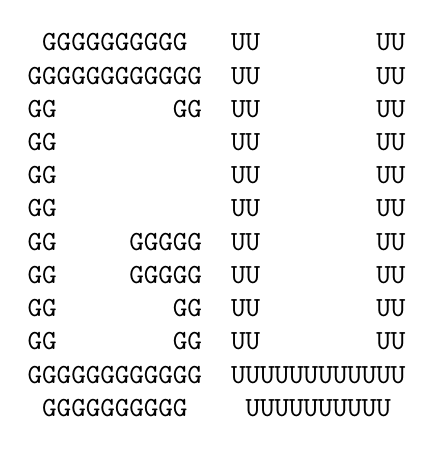
\begin{tikzpicture}
\node[anchor=west,inner sep=0pt] {\ttfamily\begin{tabular}{@{}l@{}}
\phantom{G}GGGGGGGGGG\phantom{GGG}UU\phantom{UUUUUUUU}UU\\
GGGGGGGGGGGG\phantom{GG}UU\phantom{UUUUUUUU}UU\\
GG\phantom{GGGGGGGG}GG\phantom{GG}UU\phantom{UUUUUUUU}UU\\
GG\phantom{GGGGGGGGGGGG}UU\phantom{UUUUUUUU}UU\\
GG\phantom{GGGGGGGGGGGG}UU\phantom{UUUUUUUU}UU\\
GG\phantom{GGGGGGGGGGGG}UU\phantom{UUUUUUUU}UU\\
GG\phantom{GGGGG}GGGGG\phantom{GG}UU\phantom{UUUUUUUU}UU\\
GG\phantom{GGGGG}GGGGG\phantom{GG}UU\phantom{UUUUUUUU}UU\\
GG\phantom{GGGGGGGG}GG\phantom{GG}UU\phantom{UUUUUUUU}UU\\
GG\phantom{GGGGGGGG}GG\phantom{GG}UU\phantom{UUUUUUUU}UU\\
GGGGGGGGGGGG\phantom{GG}UUUUUUUUUUUU\\
\phantom{G}GGGGGGGGGG\phantom{GGGG}UUUUUUUUUU
\end{tabular}};
\end{tikzpicture}}

% printed form: six repeated lines on the reverse; the last field is cut by the edge
\begin{tabular}{@{}l@{}}
\texttt{*P\quad END\quad STC\quad 124\quad GUTS\quad 0070 0001 M06}\quad\illegible{3}\quad\unsure{MOR|MOB}\\
\texttt{*P\quad END\quad STC\quad 124\quad GUTS\quad 0070 0001 M06}\quad\illegible{3}\quad\unsure{MOR|MOB}\\
\texttt{*P\quad END\quad STC\quad 124\quad GUTS\quad 0070 0001 M06}\quad\illegible{3}\quad\unsure{MOR|MOB}\\
\texttt{*P\quad END\quad STC\quad 124\quad GUTS\quad 0070 0001 M06}\quad\illegible{3}\quad\unsure{MOR|MOB}\\
\texttt{*P\quad END\quad STC\quad 124\quad GUTS\quad 0070 0001 M06}\quad\illegible{3}\quad\unsure{MOR|MOB}\\
\texttt{*P\quad END\quad STC\quad 124\quad GUTS\quad 0070 0001 M06}\quad\illegible{3}\quad\unsure{MOR|MOB}
\end{tabular}
\scanpage{434}
\mspage{1}
% archive sheet number: 433

Intégration des 1-types d'homotopie relatifs sur une catégorie.

Les types d'homotopie relatifs sur une (petite) catégorie $S$ sont définis par les \uline{champs} \inserted{(en cat.)} sur $\hat S$, qui correspondent essentiellement aux contrafoncteurs $S^{\unsure{\circ|o}}\unsure{\mathrel{-}|\longrightarrow}(\mathrm{Cat})$, ou encore aux catégories $X$ sur $S$ qui sont Cat-fibrées sur $S$. \inserted{(Dans $(\mathrm{Cat}\deleted{\unsure{\mathrm{fib}}}/S)_{\mathrm{fib}}$, on inverse les flèches qui sont des Hot-équiv. sur les fibres.)}

D'autre part, les 1-types d'homotopie relatifs sur $S$ doivent se décrire par des \uline{champs en groupoïdes} sur $S$.

Si \deleted{\unsure{$S$}} on a un type d'homotopie relatif, défini par

\[
\begin{aligned}
X&\longrightarrow S & &\text{cat. Cat-fibrée sur }S\\
&&&\text{ou par}\quad S^\circ\longrightarrow\mathrm{Cat}\\
&&&& s\longmapsto X_s,
\end{aligned}
\]

le 1-type d'homotopie associé est défini par

\[
s\longrightarrow\Pi(X_s)\qquad S^\circ\longrightarrow(\mathrm{Gr}\unsure{p|po}\deleted{\unsure{\mathrm{d}}})
\quad\substack{\text{cat. des}\\\text{groupoïdes}}
\]

où $\Pi(X_s)$ est le groupoïde fondamental de $X_s$. \deleted{\unsure{Il est}} \inserted{\unsure{Je}} note la \deleted{\illegible{1}} cat. fibrée correspondante sur $S$ par $\boxed{\Pi(X/S).}$ Il est \unsure{vrai} \deleted{\unsure{vrai}} que si

\[
X\longrightarrow X'
\]

est une flèche de cat. fibrées \inserted{sur $S$} qui \unsure{induit|induise} une Hot-équiv sur les fibres, elle induit une équivalence fibrée \deleted{sur}

\[
\Pi(X/S)\longrightarrow\Pi(X'/S),
\]

mais non un iso. Il y \unsure{aura|a}\deleted{\unsure{it|urait}} donc du travail à faire pour \deleted{\unsure{associer à} tout type d'homotopie relatif} \inserted{définir un foncteur}

\diagram{\begin{tikzcd}[ampersand replacement=\&,column sep=12mm]
\underbrace{\unsure{\mathrm{HOT}|\mathrm{Hot}}(S)}_{\substack{\text{cat. des}\\\text{types d'hom}\\\text{relatifs sur }S}}
\arrow[r,"{\unsure{\xi|\zeta}\mapsto\Pi(\unsure{\xi|f|\vert}/S)}"] \&
\underbrace{\uline{\mathrm{Grp}}(S)}_{\substack{\text{catégorie des}\\\text{groupoïdes}\\\deleted{\unsure{f}}\text{fibrés sur }S\\
\text{(ou cat. des}\\\text{champs en groupoïdes}\\\text{sur }\hat S\text{)}}}
\end{tikzcd}}

Mais ce n'est pas pour l'instant mon propos. Plutôt de donner une formule de transitivité \inserted{en homotopie} \unsure{ou où on voit bien|ou ce qui serait bien} \deleted{\illegible{1}} \inserted{\unsure{analogue à}} $R(gf)_*\simeq Rg_*Rf_*$ en cohomologie.
\scanpage{435}
\mspage{2}
% archive sheet number: 434

Si

\[
f\colon S\unsure{\mathrel{-}|\longrightarrow}T
\]

est un foncteur, \deleted{\unsure{tout}} on va définir un foncteur

\[
f_!\colon\uline{\mathrm{Grp}}(S)\longrightarrow\uline{\mathrm{Grp}}(T)
\]

(image directe de 1-types d'homotopie relatifs) Mais notons d'abord que si

\[
p\colon X\longrightarrow S
\]

est une $S$-catégorie \uline{quelconque} (pas néc. Cat-fibrée), on \unsure{peut associer|lui associe} néanmoins un type d'hom relatif, via la catégorie fibrée \inserted{$\widetilde X^{\unsure{(S)|S}}$ ou $\widetilde X$} ayant comme fibres les ${}_{s}\backslash X$ (en notant que $s'\longrightarrow s$ dans $S$ définit bien ${}_{s}\backslash X\longrightarrow {}_{s'}\backslash X$). \deleted{\unsure{Si $X$ est déjà}} On a un $S$-foncteur canonique

\margin{Ayant $\widetilde X$, on \unsure{peut définir|définit} $\Pi(X/S)\overset{\text{déf}}{=}\Pi(\widetilde X/S)$.}
% slanted

\[
X\xrightarrow{i}\widetilde X\qquad
x\longmapsto\bigl(x,p(x),\underset{\text{``}s\text{''}}{\deleted{\unsure{p'}}p(x)}\xrightarrow{\mathrm{id}}p(x)\bigr).
\]

\deleted{qui} C'est une $S$-\inserted{Hot-}équivalence si $X$ \unsure{était} déjà fibrée. -- En fait, en chaque fibre c'est un \deleted{\unsure{équivalé}} \unsure{homotopisme}, car on construit alors $\widetilde X_{s_0}\xrightarrow{j}X_{s_0}$ de façon évidente, de façon que

\diagram{\begin{tikzcd}[ampersand replacement=\&,column sep=12mm]
X_{s_0}\arrow[r,shift left,dash,"i"] \& \widetilde X_{s_0}\arrow[l,shift left,"j"]
\end{tikzcd}}

$ji\simeq\mathrm{id}$, $ij\xrightarrow[\text{\unsure{simple}}]{\text{homotopie}}\mathrm{id}$ (NB cette flèche n'est pas iso en général.)

Revenons alors à $f\colon S\longrightarrow T$, et considérons un groupoïde fibré sur $S$

\[
G\longrightarrow S,
\]

ce n'est pas une catégorie fibrée sur $\deleted{\unsure{S}}T$, \deleted{\unsure{p}} mais on peut lui associer

\[
t\longmapsto {}_{t}\backslash G\qquad T^{\unsure{\circ|o}}\unsure{\mathrel{-}|\longrightarrow}(\mathrm{Cat}),
\]

d'où une catégorie fibrée sur $T$, dont on prend le $\Pi$ relatif. Mais il est plus simple de prendre \deleted{les} \inserted{\unsure{directmt|directement}}

\[
t\longmapsto\Pi({}_{t}\backslash G)
\]

qui \deleted{\unsure{est}} \inserted{définit} une \deleted{\unsure{champ}} catégorie fibrée en groupoïdes sur $S$.
\scanpage{436}
\mspage{3}
% archive sheet number: 435

Ainsi on trouve bien un foncteur (en fait, \unsure{$=$|même} un 2-foncteur de 2-catégories)

\[
f_!\colon\uline{\mathrm{Grp}}(S)\longrightarrow\uline{\mathrm{Grp}}(T)
\]

Si

\[
u\colon G\longrightarrow G'
\]

est un \unsure{hom|lien} de groupoïdes fibrés sur $S$, qui induise \deleted{des} \inserted{Cat-}équivalences sur les fibres, alors

\[
f_!(u)\colon f_!(\unsure{G|u})\unsure{\mathrel{-}|\longrightarrow}f_!(G')
\]

est aussi une Cat-équiv sur les fibres. (Cela est formel, à partir du fait que $f_!$ est un 2-foncteur, compte tenu que si on a une équiv. $u$ sur les fibres, alors il y a un quasi-inverse -- c'est une histoire générale de cat. fibrées\ldots)

Soit maintenant

\[
p\colon X\longrightarrow S,
\]

et prenons le cas $G=\Pi(X/S)$. Je dis qu'on a alors une \uline{$T$-équivalence} \unsure{can}

\[
\boxed{f_!\bigl(\Pi(X/S)\bigr)\simeq\deleted{\unsure{g}}\Pi(X/T)}
\]

en d'autres termes, pour connaître $\Pi(X,T)$ \inserted{(à $T$-équiv près)}, il suffit de connaître $\Pi(X/S)$, et de lui appliquer le foncteur $f_!$ d'intégration des 1-types d'homotopie relatifs, pour $f\colon S\longrightarrow T$.

Notons que l'on a trivialement

\[
\Pi(X/S)=p_!(\unsure{e}_X)
\]

où $e_X$ désigne le $X$-groupoïde fibré trivial (toutes les fibres ponctuelles). Donc la formule précédente s'écrit comme une formule de transitivité

\[
f_{\deleted{\unsure{*}}!}\bigl(p_!(\unsure{\Pi|\Gamma|\mathscr T})\bigr)\simeq(fp)_!(\unsure{\Gamma|\mathscr T|\mathrm{I}}),
\]
\scanpage{437}
\mspage{4}
% archive sheet number: 436

où $\unsure{\Gamma|\mathscr T}$ est le groupoïde fibré trivial sur $X$. Cela suggère de généraliser la formule \unsure{cas|bis} en

\[
\boxed{(fp)_!(\unsure{\Gamma|\Gamma'|C})\simeq f_!(p_!(\Gamma))}
\]

pour \uline{tt} groupoïde fibré sur $X$, dans une situation

\[
X\xrightarrow{p}S\xrightarrow{f}T.
\]

Ce sera formel si on établit une propriété \unsure{de|d'} \inserted{2-}adjonction pour le foncteur $f_!$ : \deleted{Soit $G$}

\uline{Th} Soit $f\colon S\longrightarrow T$ une \deleted{foncteur} flèche dans $(\mathrm{Cat})$, $G$ un champ en groupoïdes sur $S$, $H$ un champ en groupoïdes sur $T$. On a alors une équivalence de catégories canonique

\[
\boxed{\uline{\mathrm{Hom}}_{\uline{\mathrm{Grp}}(S)}(G,f^*H)
\simeq\uline{\mathrm{Hom}}_{\uline{\mathrm{Grp}}(T)}(f_!G,H)}
\]

Les flèches d'adjonction

\[
\left\{\begin{aligned}
f_!f^*H&\longrightarrow H & H&\in\mathrm{Ob}\,\uline{\mathrm{Grp}}(T)\\
f^*f_!G&\longleftarrow G & G&\in\mathrm{Ob}\,\uline{\mathrm{Grp}}(S)
\end{aligned}\right.
\]

devraient se définir sans problème. Pour la dernière, il faut définir pour $s\in S$

\[
G_s\longrightarrow(f^*(f_!G))_s=(f_!(G))_{f(s)}
\overset{\text{déf}}{=}\Pi({}_{s}\backslash G)
\]

or on a

\[
G_s\longrightarrow {}_{s}\backslash G\qquad\text{d'où}
\]

\diagram{\begin{tikzcd}[ampersand replacement=\&,row sep=2mm]
\& \Pi(G_s)\arrow[r]\arrow[d,equals]\arrow[dl,bend right=9] \& \Pi({}_{s}\backslash G),\\
\substack{\text{car }G_s\text{ est}\\\text{un groupoïde}} \& G_s \&
\end{tikzcd}}

OK, C'est fonctoriel en $s$ \unsure{\ldots}.
\scanpage{438}
\mspage{5}
% archive sheet number: 437

Pour la flèche $f_! f^{\unsure{\prime|*}}H\longrightarrow H$ sur $T$, il faut trouver pour \unsure{tt} $t\in\mathrm{Ob}\,T$, et fonctoriellement en $t$

\diagram{\begin{tikzcd}[ampersand replacement=\&,row sep=4mm]
\underset{\raisebox{0pt}{\rule{.35pt}{.5ex}\rule{3.5em}{.35pt}\rule{.35pt}{.5ex}}}{(f_!f^*H)_t}\arrow[r]\arrow[d,equals,"\mathrm{def}"] \& H_t\arrow[d,equals]\\
\Pi({}_{t}\backslash f^*(H)) \& \Pi(H_{\unsure{t|f}})
\end{tikzcd}}

il suffirait donc de définir

\[
{}_{t}\backslash f^*(H)\longrightarrow H_t,
\]

mais \deleted{\unsure{avec} le diagramme cartésien}

\diagram{\begin{tikzcd}[ampersand replacement=\&,column sep=12mm]
f^*H=H\times_S T\arrow[r,dash]\arrow[d] \& H\arrow[d]\\
S\arrow[r,dash,"f"] \& T\ni t
\end{tikzcd}}

\unsure{induisant|s'en déduit} $f^*H\unsure{\mathrel{-}|\longrightarrow}H$ d'où

\[
\deleted{f^*(H)_t=S_{\unsure{t|f}}\times H_t\xrightarrow{\mathrm{pr}_2}H_t}
\]

\deleted{d'autre part on a}

\[
\deleted{f^*(H)_t\longrightarrow {}_{t}\backslash f^*(H)}
\]

\[
{}_{t}\backslash f^*(H)\longrightarrow {}_{t}\backslash H
\qquad\substack{\text{(au lieu de s'envoyer}\\\text{dans }H_t\text{)}}
\]

mais d'autre part, comme \unsure{$H$|tout} est fibrée sur $T$ donc lisse sur $T$, l'inclusion

\[
\deleted{\unsure{t}}H_t\longrightarrow {}_{t}\backslash H
\]

est une Hot-équivalence. Ou disons plutôt : $f^*H\longrightarrow H$ est un morphisme de catégories sur $T$, induisant

\diagram{\begin{tikzcd}[ampersand replacement=\&,row sep=3mm]
\deleted{\unsure{f_!(f)}}\Pi(f^*H/T)\arrow[r]\arrow[d,equals,"\mathrm{def}"] \& \Pi(H/T),\\
f_!(f^*H) \&
\end{tikzcd}}
\scanpage{439}
\mspage{6}
% archive sheet number: 438

or le \inserted{$T$-}foncteur canonique

\[
H\longrightarrow\Pi(H/T)\qquad
\substack{\text{(= cat. sur }T\text{ définie}\\
\text{par }\ t\longmapsto\Pi({}_{t}\backslash H)}
\]

est une \deleted{\unsure{$S$}} équivalence, puisque $H$ est un \deleted{groupoïde} fibré en groupoïdes sur $T$. Donc on peut \deleted{\unsure{l'inverser en}} trouver un \inserted{$T$-}quasi-inverse

\[
\Pi(H/T)\longrightarrow H
\]

et en composant on trouve

\[
f_!(f^*H)\longrightarrow\Pi(H/T)\unsure{\mathrel{-}|\longrightarrow}H
\]

la flèche cherchée.

Ayant les \inserted{\unsure{2|2\textsuperscript{e}}} flèches d'adjonction, je m'arrête là dans les vérifications !

\unsure{Questions|Question} de changement de base

\diagram{\begin{tikzcd}[ampersand replacement=\&,column sep=8mm,row sep=6mm]
\& G \& {} \& {}\\
\& S\arrow[d,"f"'] \& S'\arrow[l,"q"']\arrow[d,"f'"] \& {}\\
(*) \& T \& T'\arrow[l,"p"] \& p^*f_!(G)\longleftarrow f'_!q^*(G)
\arrow[from=3-3,to=2-2,shorten <=5mm,shorten >=6mm,"\unsure{\gamma|r}"]
\end{tikzcd}}

La flèche est définie, pourvu qu'on ait commutativité \inserted{\unsure{ou} une flèche de commutativité $\gamma\colon pf'\unsure{\mathrel{-}|\longrightarrow}fq$ (pas néc. iso).} \deleted{\unsure{Par}} Par adjonction, il revient au \unsure{$=$|même} de donner

\diagram{\begin{tikzcd}[ampersand replacement=\&,column sep=11mm,row sep=5mm]
p_!f'_!q^*G\arrow[r,dash]\arrow[d,"\text{transitivité}"',"\simeq",dash] \& f_!(G)\\
(pf')_!q^*G\arrow[d,"\gamma"] \& {}\\
(fq)_!q^*G\arrow[uur,"\text{car }q_!q^*G\longrightarrow G"'] \& {}\\
f_!(q_!q^*)G\arrow[u,"\text{transitivité}"',"\simeq",dash] \& {}
\end{tikzcd}}

On se demande quand la flèche est iso.
\scanpage{440}
\mspage{7}
% archive sheet number: 439

Le théorème suivant doit être vrai, et résulter de \unsure{mes} fourbis généraux.

\uline{Théorème} Si le \deleted{\unsure{morphisme}} carré $(*)$ est \uline{cartésien} \inserted{\unsure{de|dans} $(\mathrm{Cat})$},

\noindent\begin{tabular}{@{}|p{.93\linewidth}@{}}
$\unsure{\gamma|r}$ \deleted{l'identité} un iso, et si on suppose que $f$ soit 1-lisse,
ou $p$ 1-propre, alors \unsure{le|la} \deleted{\unsure{signe}} $T'$-foncteur de
changement de base est une \unsure{équivalence} de \inserted{$T'$-}cat..
\end{tabular}

Les ``fourbis'' généraux seraient \deleted{\unsure{serait}} en termes \deleted{\unsure{termes}} d'un dérivateur $\unsure{\mathbb D|\mathrm D}$ ad hoc, celui des 1-types d'homotopie relatifs.. J'y reviendrai par la suite.

On se pose la question quand le 2-foncteur associé à \deleted{\unsure{$f$}} $f\colon S\longrightarrow T$

\[
f^*\colon\uuline{\mathrm{Grp}}(T)\unsure{\mathrel{-}|\longrightarrow}\uuline{\mathrm{Grp}}(S)
\]

est 0-fidèle, 1-fidèle, 2-fidèle, \deleted{\unsure{i.e.}} \deleted{Cela} Si $G,H$ sont \deleted{des} \unsure{gr|g} fibrés en groupoïdes sur $T$, on considère

\margin{La \unsure{$i$-fidélité|$i$-infidélité} de $f^*$ ($i\in\{\deleted{\unsure{n}},0,1,2\}$) équivaut à celle des foncteurs (obtenus \deleted{\unsure{à|en}} en prenant $G=e_T$) $\uline{\unsure{\Gamma|\mathscr T}}(H/T)\longrightarrow\uline{\Gamma}(f^*H/S)$.}
% slanted

\[
\uline{\mathrm{Hom}}_{\uuline{\mathrm{Grp}}(T)}(G,H)\unsure{\mathrel{-}|\longrightarrow}
\uline{\mathrm{Hom}}_{\uuline{\mathrm{Grp}}(S)}(f^*G,f^*H),
\]

et suivant que ce foncteur est toujours fidèle, ou pleinement fidèle, ou une équivalence de cat on dit que $f^*$ est 0-, 1-, ou 2-fidèle. Dans le cas 2-fidèle, cela \deleted{signifie} \inserted{implique} que si $K$ est un fibré en groupoïdes sur $S$, s'il est équivalent à un $f^*G$, alors $G$ est déterminé à \inserted{$T$-}équiv. près, elle \unsure{$=$|même} déterminée à iso unique près, \deleted{Si ça marche pour \uline{tt} $K$, je dirai que $f^*$ est 3-fidèle. On veut des critères \unsure{commodes} \deleted{pour} \deleted{\unsure{que ce soit}} de la $i$-fidélité.}
\scanpage{441}
\mspage{8}
% archive sheet number: 440

\inserted{Soit $i\in\mathbb N$} On dit que $f$ est $i$-\uline{asphérique} si $\forall\,\unsure{t|s}\in\unsure{T|S}$, $Z=S/t$ est $i$-asphérique, \deleted{\illegible{1}} i.e. a $\pi_0(Z)\mathrel{-}\pi_i(Z)$ triviaux. On définit aussi $(-1)$-asphérique : les $S/t$ sont non vides. De \unsure{$=$|même} pour la notion de $i$-coasphérique.

\deleted{On doit avoir le\par \uline{Théorème ?} \inserted{Soit $f\colon S\longrightarrow T$ dans Cat, $i\in[\unsure{-0|0},\unsure{2|3}]=\{0,1,2,\deleted{\unsure{3}}\}$} a) Si $f$ est $(i-1)$-asphérique \inserted{et $(i-1)$-propre} ou \unsure{resp.} coasphérique \deleted{et de plus, lisse ou propre, (il suffit} $(i-1)$-lisse, \deleted{\unsure{ou $(i-1)$-propre})} alors le foncteur $f^*$ précédent est \deleted{\unsure{($i$}}\unsure{$i$}-fidèle. \par b) Supposons $f^*$ 2-fidèle, et soit $G$ un \deleted{\unsure{group}} fibré en groupoïdes sur $S$. Pour que $G$ soit $S$-équivalent à un \deleted{fibré en groupoïdes} $f^*(H)$, il \unsure{f.|faut} et s. que ce soit vrai \inserted{\unsure{colocalement|localement}} localement sur $T$}

En fait, pour $i\in[-1,+\infty[\ \subset\mathbb Z$, on définit un dérivateur $\unsure{\mathbb D|\mathrm D}_i$ des $i$-types d'homotopie relatifs (cf plus bas). D'où les notions d'objet $\mathbb D_i$-asphérique ($=i$-asphérique), de $\mathbb D_i$-équivalence, de foncteurs $\mathbb D_i$-asphériques et $\mathbb D_i$-coasphériques, de foncteurs $\mathbb D_i$-lisses et $\mathbb D_i$-propres, de $\mathbb D_i$-fibrations et de $\mathbb D_i$-\unsure{cofibrations|fibrations} \uline{triviales} \deleted{\unsure{dont}} (i.e. à fibres $\mathbb D_i$-asphériques). On doit avoir le

\uline{Théorème ?} Soit $f\colon S\longrightarrow T$ dans $(\mathrm{Cat})$, $i\in\{0,1,2\}$. \deleted{\unsure{a)}} \deleted{\unsure{Si $f$ est}} Supposons l'une des conditions suivantes \unsure{satisfaite|satisfaites} :

a) $f$ est $(i-1)$-propre, et $(i-1)$-asphérique (s'exprime par la condition que certaines catégories, telles les $S/t$, soient $(i-1)$-asphériques)

b) $f$ est $(i-1)$-lisse, et $(i-1)$-coasphérique.

Alors \textcircled{1} le foncteur $f^*$ d'image inverse

\[
f^*\colon\uline{\mathrm{Grp}}(T)\unsure{\mathrel{-}|\longrightarrow}\uline{\mathrm{Grp}}(S)
\]

est $i$-fidèle. \textcircled{2} Dans le cas $i=2$ ($f^*$ pl. fidèle) on
\scanpage{442}
\mspage{9}

a de plus ceci : si $G\in\mathrm{Ob}\,\uline{\mathrm{Grp}}(S)$ est un fibré en groupoïdes sur $S$, alors $G$ est équivalent à un fibré en groupoïdes de la forme $f^*(H)$ sss \deleted{\unsure{il existe|il est}} \inserted{pour} tout $t\in T$, la restriction \inserted{$G_t$} de $G_{\deleted{\unsure{t|s}}}$ à $\deleted{\unsure{T}}S_t$ \unsure{soit|est} équivalente à un \inserted{fibré en} groupoïdes constant sur $\deleted{\unsure{T}}S_t$. (\uline{NB} les conditions a) ou b) impliquent déjà que $S_t$ est $1$-connexe, i.e. que son groupoïde fondamental est \unsure{équiv.|équiv} à $e$.)

\textcircled{3} Soit $Z$ un objet $1$-connexe dans $(\mathrm{Cat})$, \deleted{Pour} $G$ un fibré en groupoïdes sur $Z$. Pour que $G$ soit \inserted{$Z$-}équivalent à un groupoïde constant sur $Z$, il \unsure{faut|f.} et s. que pour \unsure{tte|toute} flèche $u$ de $Z$, \deleted{\unsure{m.s.|m.s}} le \deleted{foncteur} morphisme de groupoïdes \unsure{cor\textsuperscript{t}|corr\textsuperscript{t}} induit sur les fibres de $G$ soit une \inserted{$Z$-}équivalence.

% slanted

\margin{On dit alors que $G$ est \uline{essentiellement} \uline{\unsure{loc.|loco.} constant} sur $Z$.}

\uline{Corollaire} La condition \unsure{trad.|trad.le} de $2^{\circ}$) s'exprime ainsi : pour toute flèche \inserted{$u$ de $S$} ``verticale'' \deleted{pour $f$} \inserted{sur $T$} i.e. telle que $f(u)$ soit une flèche identique, le foncteur $u^*$ induit \unsure{par} $u$ sur les fibres de $G$ soit une équivalence de groupoïdes

% archive sheet number: 441
